\section{Introduction}
\label{sec:introduction}

% state the learning objective 
The objective of this laboratory assignment is to create a AC/DC Converter, a circuit that converts alternate current into direct current, and then, analyse it. This converter is composed by an envelope detector and a voltage regulator.

As seen in Figure \ref{fig:rc}, this circuit can be divided in four parts: \textbf{Voltage Source}, which has an amplitude of 230 V and a frequency of 50 Hz; \textbf{Transformer}, used to transform the supplied voltage into a lower voltage; \textbf{Envelope Detector}, which includes a full wave bridge rectifier and a capacitor ;\textbf{Voltage Regulator}, which consists of a capacitor, a resistor and also a limiter - 25 diodes in series.

\begin{figure}[h] \centering
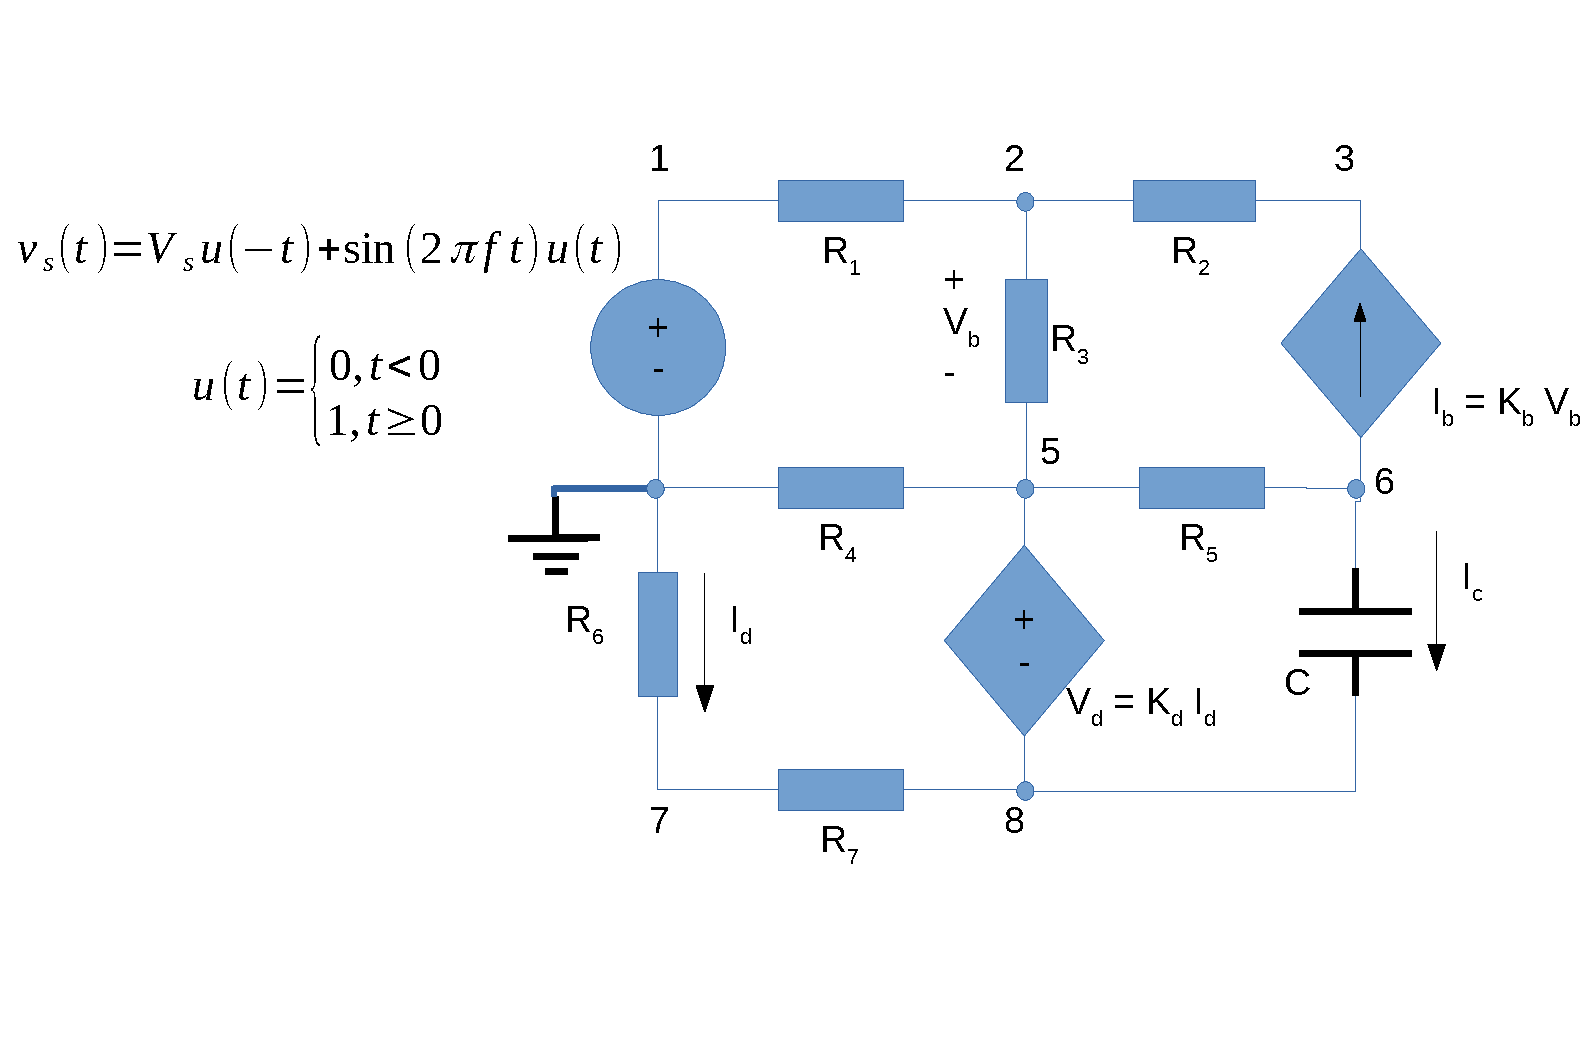
\includegraphics[width=0.99\linewidth]{rc.pdf}
\vspace{-5mm}
\caption{The AC/DC converter}
\label{fig:rc}
\end{figure}






